\documentclass{article}
\pagenumbering{arabic}


\newcommand{\newCommandName}{text to insert}
% Pages and colors used for the cover page
\usepackage{tikz-page}
\usepackage{url}
\usepackage{lastpage}

% Used for the math and code
\usepackage{amsmath}
\usepackage{listings}
\usepackage{pythonhighlight} % Got this from github! https://github.com/olivierverdier/python-latex-highlighting/blob/master/pythonhighlight.sty

% Used for the pictures
\usepackage{float}
\usepackage{graphicx}

% For the table
\usepackage[utf8]{inputenc}
\usepackage{multirow}
\usepackage{colortbl}
\usepackage{nicematrix}
\usepackage{tabularray}


% for blue urls
\usepackage{xcolor}
\usepackage[normalem]{ulem}
\usepackage{hyperref}
\hypersetup{colorlinks,urlcolor=blue}
%% or
% \hypersetup{colorlinks=false,pdfborder=000}

% hack into hyperref
\makeatletter
\DeclareUrlCommand\ULurl@@{%
  \def\UrlFont{\ttfamily\color{blue}}%
  \def\UrlLeft{\uline\bgroup}%
  \def\UrlRight{\egroup}}
\def\ULurl@#1{\hyper@linkurl{\ULurl@@{#1}}{#1}}
\DeclareRobustCommand*\ULurl{\hyper@normalise\ULurl@}
\makeatother



\usepackage[
  top=2cm,
  bottom=2cm,
  left=3cm,
  right=2cm,
  headheight=17pt, % as per the warning by fancyhdr
  includehead,includefoot,
  heightrounded, % to avoid spurious underfull messages
]{geometry} 

% Page numbers/header
\usepackage{fancyhdr}
\definecolor{brickred}{rgb}{0.8, 0.25, 0.33}
\definecolor{cobalt}{rgb}{0.0, 0.28, 0.67}
\definecolor{cadetgrey}{rgb}{0.57, 0.64, 0.69}

% Defining the text box being used for DEPT OF ENG
\tikzset{
        secnode/.style={
                minimum height = .16in,
                minimum width = 4.16in,
                inner xsep = 2pt,
                anchor=north east,
                draw=cadetgrey,
                fill=white,
                text=brickred,
                },
        }


         
\pagestyle{plain}
\renewcommand{\headrulewidth}{0pt}


\begin{document}


% Put name data and assignment number here
\newcommand\personaldate{April 29, 2024}
\newcommand\myname{Jonathan Isely, Jalen Guan, Leo Berman, Yuan Nghiem, Jake Grinshpun}
\newcommand\myemail{Jonathan.Isely@temple.edu, Jialiang.Guan@temple.edu, Leo.Berman@temple.edu, Yuan.Nghiem@temple.edu, Jacob.Grinshpun@temple.edu }
\newcommand\mynameabbrev{J. Isely, J. Guan, L. Berman, Y. Nghiem, J. Grinshpun}
\newcommand\assignmenttitle{Multi-Room Light Usage Analysis Web App}
\newcommand\yourclass{ECE 3824: Computation III}
\begin{titlepage}
	% Drawing the border and the text box 
	\newcommand{\tikzpagelayout}{
		\draw[line width = .04in,
			color = cobalt]
		($(current page.north west)+(1in,-1in)$)
		rectangle ($(current page.south east)+(-.625in,1in)$);

		\draw[line width = .04in,
			color = brickred]
		($(current page.north west)+(.92in,-.92in)$)
		rectangle ($(current page.south east)+(-.705in,1.08in)$);
		\node[secnode] at ($(current page.north west)+(6in,-.875in)$) {\small{\textbf{DEPARTMENT OF ELECTRICAL AND COMPUTER ENGINEERING}}};
	}

	\begin{center}
		\large{\textbf{\assignmenttitle}}\break
		\break
		\large{submitted to \:}\break
		\large{Professor Iyad Obeid}\break\break
		\large{ECE 3824: Computation III}\break
		\large{Temple University}\break
		\large{College of Engineering}\break
		\large{1947 North 12th Street}\break
		\large{Philadelphia, Pennsylvania 19122}\break
		\break
		\large{\personaldate}\break
		\break
		\large{Prepared by: }
		\large{\myname}\break\break
		\large{Emails: \myemail}\break
	\end{center}
\end{titlepage}

\newpage
\pagestyle{fancy}
\fancyhead{}
\fancyfoot{}
\fancyhead[R,EH]{Page \thepage\ of \pageref{LastPage}}
\fancyhead[L,EH]{\mynameabbrev}
\fancyfoot[L,EF]{\yourclass}
\fancyfoot[R,EF]{\personaldate}
\renewcommand{\thesection}{\Alph{section}.}

\section{GOAL}
\begin{flushleft}
  The goal of our project was to develop a system that does the following:
  \begin{itemize}
    \item Hardware component that checks the status of the room lights
    \item Database for our hardware component to store its results
    \item Backend to connect all components
    \item User-friendly website for our database to be searched 
  \end{itemize}

\end{flushleft}
\section{HARDWARE COMPONENT}
\begin{flushleft}
  Our hardware component requirements:
  \begin{itemize}
    \item Monitor a voltage in pin and make decisions
    \item Access the internet and make requests
  \end{itemize}
  The ESP32, in conjunction with a light sensor module, is a relatively inexpensive option that fulfills all of our requirements.\break
\begin{figure}[H]
        \centering
        \begin{minipage}{.4\textwidth}
                        \centering
                        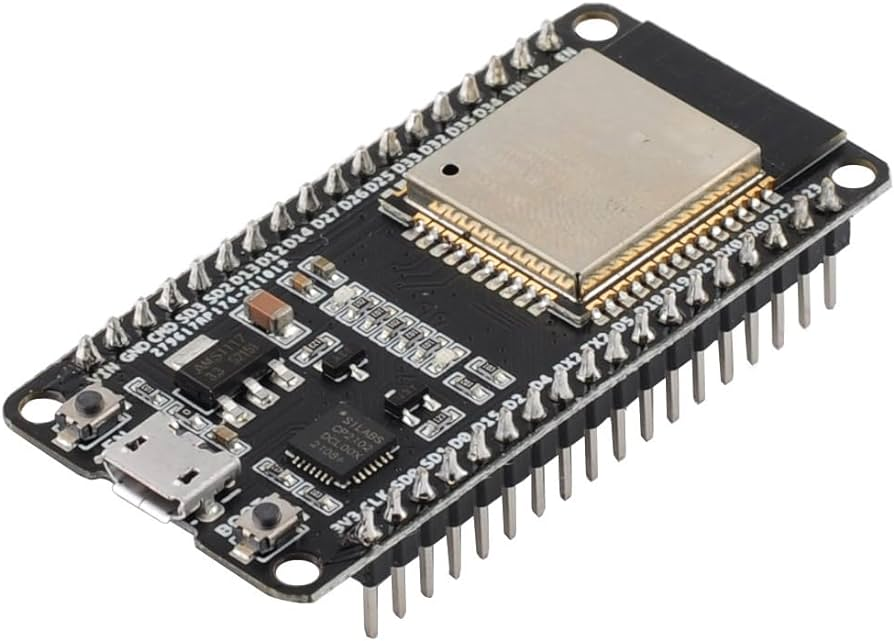
\includegraphics[height=1\linewidth]{./media/ESP32.jpg}
                        \caption{ESP32}
        \end{minipage}\hfill
        \centering
        \begin{minipage}{.4\textwidth}
                        \centering
                        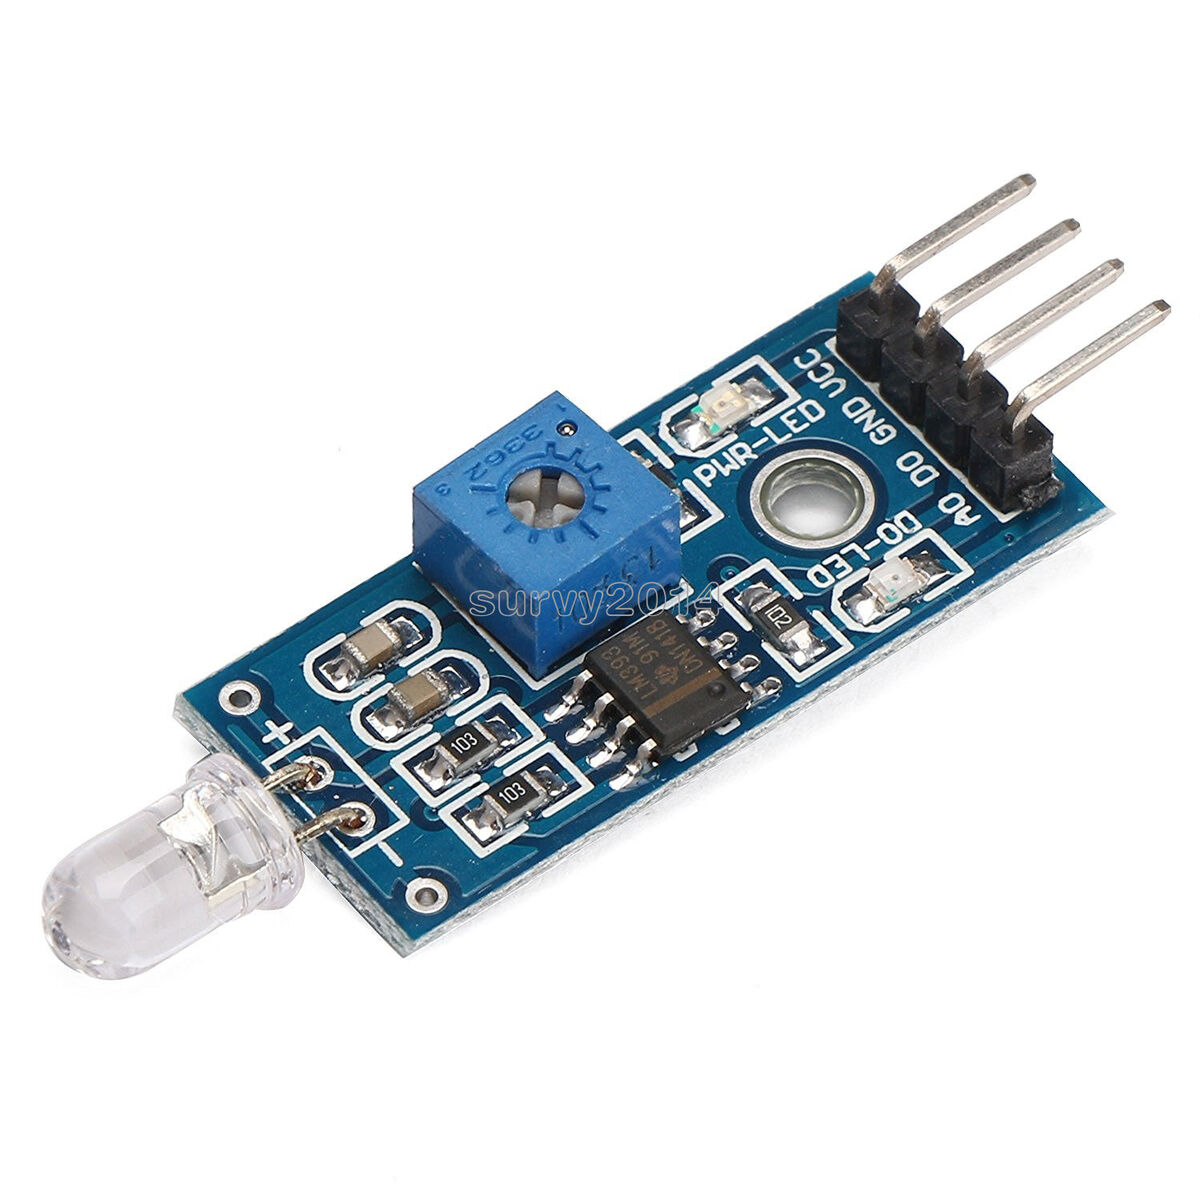
\includegraphics[height=1\linewidth]{./media/LightSensor.jpg}
                        \caption{Light Sensor}
        \end{minipage}\hfill
        \centering

\end{figure}

\end{flushleft}
\pagebreak
\section{DATABASE COMPONENT}
\begin{flushleft}
Our database component requirements:
\begin{itemize}
  \item Multi index searching using room and date/time
  \item Date/Time granularity to the minute
  \item Quick-return on multi-query requests for graphics purposes
\end{itemize}
We ended up using Amazon RDS to host a MySQL instance with one vCPU, 2 GiB of memory, 20 GiB of SSD storage. Due to the short-term nature of our system, we chose an OnDemand pricing model with RDS Proxy to minimize disruptions and increase scalability for future use of the application.\break\break

Schema with hour entries as minutes the light is on:
\begin{figure}[H]
\begin{center}
  \begin{tblr}{
  colspec = {X[c]X[c]X[c]X[c]X[c]X[c]},
  stretch = 0,
  rowsep = 6pt,
  hlines = {black, 1pt},
  vlines = {black, 1pt}
    }
    SCHEMA & room & date\_entry & hour0 & hour1 & ... & hour23\\
    SAMPLE & 603 & 2024-04-10 & 1 & 2 & ... & 3\\
    \end{tblr}
\end{center}
\caption{Schema Example}
\end{figure}
\end{flushleft}

\section{BACKEND}
\begin{flushleft}
Backend requirements:
\begin{itemize}
\item Dynamic web templating for ease of future maintenance.
\item SQL querying
\end{itemize}
A Python webapp using Flask and Jinja2 is a current industry standard that we were able to utilize. hosting on Google Cloud's App Engine, allows us to host our backend and frontend virtually free of charge.\break\break
Defining our requests using the following format:
\begin{figure}[H]
\begin{python}
    @app.route("/date")
    def date():
        ...
        return render_template('date.html')
    
    @app.route("/increment_column")
    def increment_column():
        ...
        return jsonify(success=True, status_code=200)

    @app.route("/")
    def index():
        ...
        return render_template('base.html')
\end{python}
\caption{Pseudo-code for Flask framework}
\end{figure}
\end{flushleft}

\pagebreak
\section{FRONTEND}
\begin{flushleft}
Our frontend requirements:
\begin{itemize}
  \item User friendly
  \item Future maintainable
  \item Aesthetically pleasing
\end{itemize}
With our frontend being hosted off of the python Flask/Jinja2 framework, HTML/CSS/JavaScript was an obvious choice that allowed us to create readable code with an aesthetically pleasing look.

\begin{figure}[H]


     

                        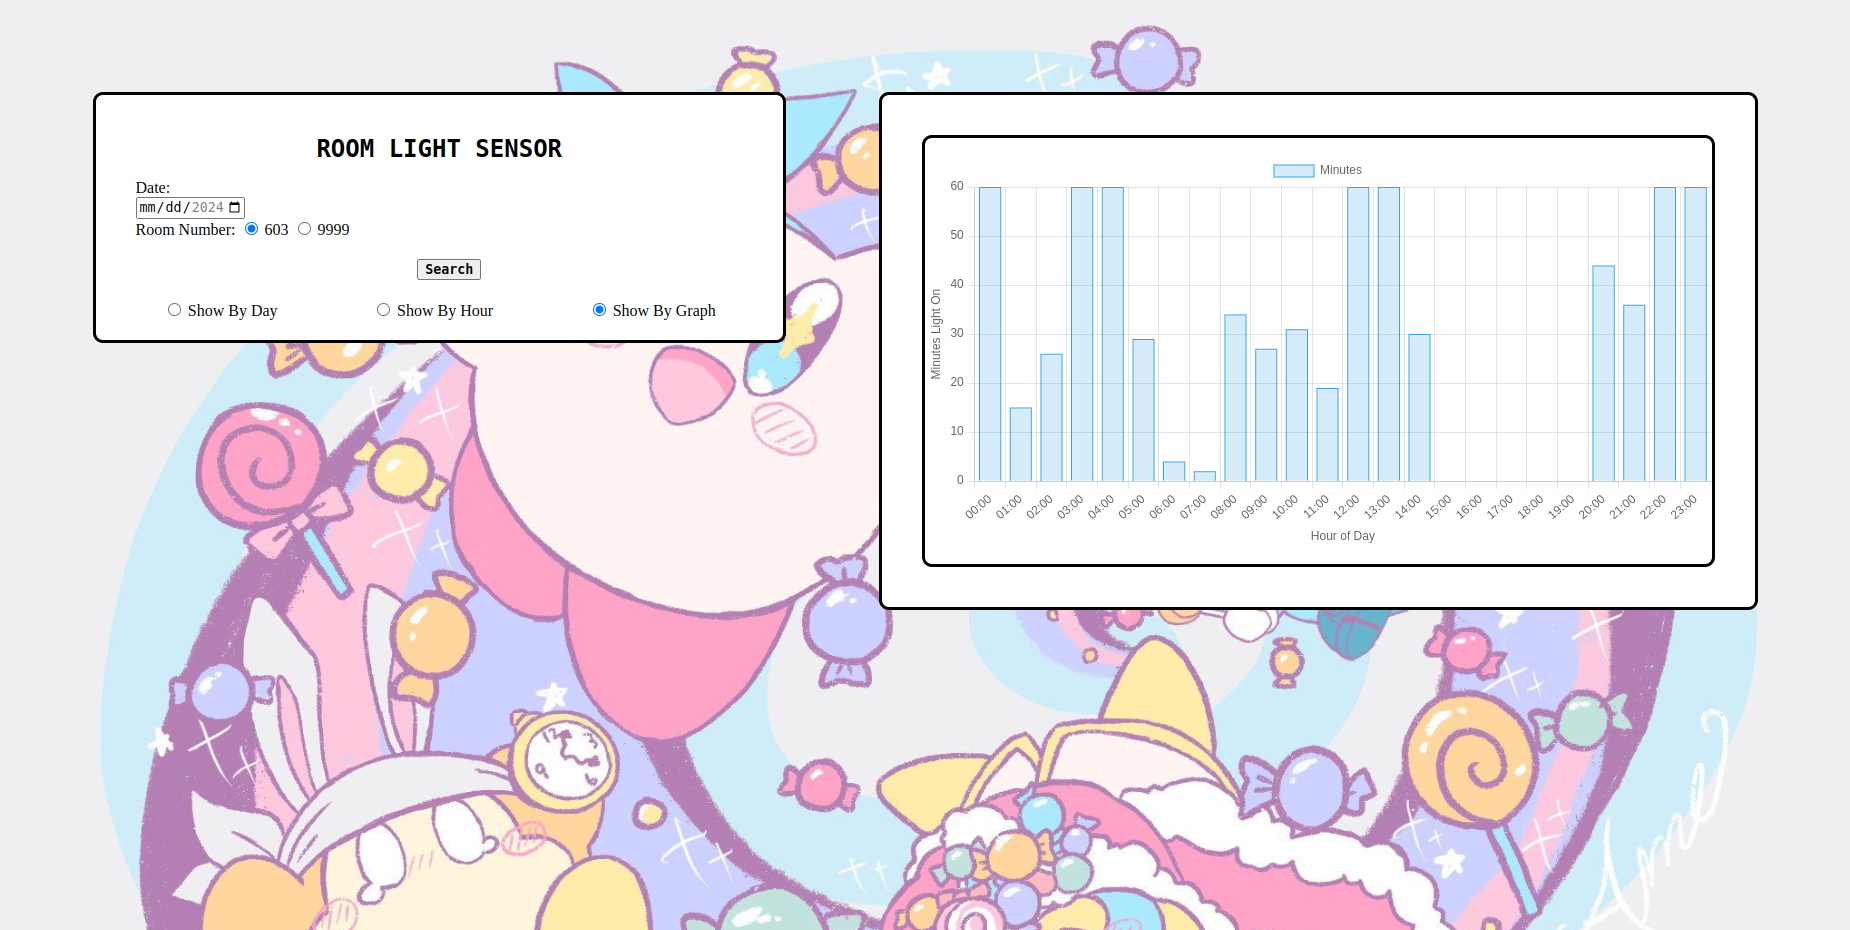
\includegraphics[height=.5\linewidth]{./media/Frontend.png}
                        \caption{Image of Web App}
     


\end{figure}

\end{flushleft}
\pagebreak
\section{COST ANALYSIS}
\begin{figure}[H]
\begin{center}
  \begin{tblr}{
  colspec = {X[c]X[c]X[c]},
  stretch = 0,
  rowsep = 6pt,
  hlines = {black, 1pt},
  vlines = {black, 1pt}
    }
    Item & Cost [\$] & Source\\
    ESP32 & 6.33 & \uline{\href{https://www.amazon.com/DORHEA-Development-Microcontroller-NodeMCU-32S-ESP-WROOM-32/dp/B086MJGFVV/ref=asc_df_B086MJGFVV/?tag=hyprod-20&linkCode=df0&hvadid=693340910094&hvpos=&hvnetw=g&hvrand=8794069933365100025&hvpone=&hvptwo=&hvqmt=&hvdev=c&hvdvcmdl=&hvlocint=&hvlocphy=9007215&hvtargid=pla-944806732492&psc=1&mcid=439cea13a85d3af483491e6e4a55da61&gad_source=4&gclid=CjwKCAjw57exBhAsEiwAaIxaZkY2bTHmsU1GMf-P4URBs-WalQ2beSx31E74vlTmGazRgUm2ybLxWRoC2UsQAvD_BwE}{Amazon Marketplace}}\\
    Light Sensor & 2.00 & \uline{\href{https://amazon.com/Oiyagai-Detection-Sensitive-Resistance-Photosensitive/dp/B09MLW5JJS/ref=asc_df_B09MLW5JJS/?tag=hyprod-20&linkCode=df0&hvadid=693270340479&hvpos=&hvnetw=g&hvrand=9988324026216616848&hvpone=&hvptwo=&hvqmt=&hvdev=c&hvdvcmdl=&hvlocint=&hvlocphy=9007215&hvtargid=pla-1929747364231&psc=1&mcid=efb7a29b544d367bb75c36ff06027577&gad_source=1&gclid=CjwKCAjw57exBhAsEiwAaIxaZpMW1T5ngkqg1tzze1ukZT_DMHsH2p2RGWoksNFA74g81Vt0oypz2xoC_gYQAvD_BwE}{Amazon Marketplace}} \\
    RDS MySQL & 24.82 / Month & \multirow{3}{*}{\uline{\href{https://calculator.aws}{Amazon Pricing Calculator}}} \\
    RDS Proxy & 21.90 / Month & \\
    RDS Storage & 2.30 / Month & \\
    \end{tblr}
\end{center}
\caption{Itemized Cost}
\end{figure}
\begin{flushleft}
Upfront Cost: \$8.33\break
Monthly Cost: \$49.02 
\end{flushleft}
\end{document}
